\section{Experimentos y Resultados}
Para la conformación del mapa de pruebas se tomó en cuenta la zona geográfica más confluida de la ciudad de Asunción, la zona céntrica, donde se concentra el ámbito empresarial, y que además posee lugares turísticos como ser el Palacio de Gobierno, la Catedral Metropolitana, la Avda. Costanera, y el casco histórico. Esta región de pruebas conforma un un grafo con 2306 vértices y 6376 aristas.

Dentro del área de trabajo definida se pudo denotar que el mismo se encontraba dentro de los cuadrantes de 6 comisarías del área metropolitana, por lo que primeramente se calculó el porcentaje de área que correspondía a cada cuadrante, luego, en base a este porcentaje fue calculado también la cantidad recursos por tipos a utilizar para las pruebas (redondeando el valor obtenido hacia el entero inferior), siendo el promedio de recursos por tipo con el que cuenta cada comisaría de 4 patrulleras, 2 motocicletas, y 3 oficiales a pie. Así, el total de recursos utilizados fue de 12 patrulleras, 5 motocicletas, y 8 oficiales. En la tabla \ref{table:calculo-recursos}, se muestran las distribuciones de recursos por cada comisaria en base a lo mencionado anteriormente.

Fueron utilizados tiempos de $T_{max}$ igual a 3 minutos y $2T_{max}$ de 6 minutos para la comparación de la metodología actual con la solución propuesta.

Para emular la metodología actual del posicionamiento de los recursos, fueron ubicados aleatoriamente cada uno de ellos dentro del cuadrante correspondiente a sus comisarias. Y para el caso de la Búsqueda Tabú como no se circunscriben las ubicaciones de los recursos dentro de la limitante de los cuadrantes, estos se ubican aleatoriamente dentro del área considerada, con la única restricción de cantidad de recursos y su cobertura intrínseca por tipo, previamente calculadas.

La presentación gráfica de los resultados cuenta con el mapa base de pruebas donde se pueden visualizar todos los tramos de la zona geográfica escogida, y un mapa de calor delictivo donde los puntos en rojo representan los lugares donde se encuentran un mayor número de tramos con niveles de violencia elevado.

En la figura \ref{fig:mapas-cobertura}, se observan con estrellas los recursos ubicados en los diferentes puntos del mapa, los trazos en verde representan los tramos que fueron cubiertos por los recursos, mientras que los trazos en negro los no cubiertos en el tiempo $2T_{max}$ por algún recurso.

El caso particular para \ref{fig:estocastico}, la distribución de los recursos no sigue ningún patrón determinado, simplemente se ubican aleatoriamente.

La tabla \ref{table:resultados-estocastico}, nos indica el valor de cobertura obtenido por cada uno de los recursos y el total de las coberturas, tanto por recurso como así en el área considerada.

En la figura \ref{fig:tabusearch}, observamos las nuevas ubicaciones basadas en la Búsqueda Tabú. Se puede observar a simple vista que la cantidad de tramos en negro es casi inexistente, indicando una cobertura casi total del área. Además de esto, también se observa cómo los recursos de mayor movilidad, los motorizados, se ubican en mayor cantidad hacia las zonas de más alto nivel de violencia, mostrado por el mapa de calor.

En la tabla \ref{table:resultados-tabu}, se denotan los valores de cobertura por cada uno de los recursos ubicados, en la cual se puede observar la particularidad de que los recursos a pie que tienen valores muy bajos e incluso cero, confirmando lo dicho anteriormente de la prioridad dada a los recursos motorizados, demostrando que la solución propuesta posee una capacidad de optimizar la ubicación priorizando la cobertura de cada tipo.

Tras las pruebas realizadas se pudo constatar que, para el área de trabajo definido los recursos no fueron suficientes para cubrir la totalidad de los tramos. Siendo el problema que la alta cantidad de tramos de accesos restrictivos superaba en gran medida la limitada cantidad de recursos a pie con los que se disponía.

\begin{table}[]
\centering
\caption{Recursos a ser utilizados, por tipo, en el área considerada.}
\label{table:calculo-recursos}
\begin{tabular}{@{}ccccccc@{}}
\toprule
\multirow{2}{*}{\textbf{Comisaría}} & \multirow{2}{*}{\textbf{Cobertura}} & \textbf{Patrulleras}                    & \multicolumn{1}{l}{} & \textbf{Motos}                          & \multicolumn{1}{l}{} & \textbf{Oficiales}                      \\ \cmidrule(lr){3-3} \cmidrule(lr){5-5} \cmidrule(l){7-7} 
                                    &                                     & \multicolumn{1}{l}{\textbf{(Prom. 4)}} & \multicolumn{1}{l}{} & \multicolumn{1}{l}{\textbf{(Prom. 2)}} & \multicolumn{1}{l}{} & \multicolumn{1}{l}{\textbf{(Prom. 3)}} \\ \midrule
\textbf{18va}                       & 33\%                                & 1                                       &                      & 0                                       &                      & 1                                       \\
\textbf{4ta}                        & 50\%                                & 2                                       &                      & 1                                       &                      & 1                                       \\
\textbf{3ra}                        & 55\%                                & 2                                       &                      & 1                                       &                      & 1                                       \\
\textbf{5ta}                        & 100\%                               & 4                                       &                      & 2                                       &                      & 3                                       \\
\textbf{9na}                        & 33\%                                & 1                                       &                      & 0                                       &                      & 1                                       \\
\textbf{21ra}                       & 50\%                                & 2                                       &                      & 1                                       &                      & 1                                       \\ \midrule
\multicolumn{2}{c}{\textbf{Total Recursos}}                               & 12                                      &                      & 5                                       &                      & 8                                       \\
\bottomrule
\end{tabular}
\end{table}
\begin{table}
\centering
\caption{Niveles de violencia cubiertos por tipo de recurso - Método aleatorio}
\label{table:resultados-estocastico}
\begin{tabular}{crrrr}
\toprule
\textbf{Recurso} & \multicolumn{1}{c}{\textbf{Patrullera}} & \multicolumn{1}{c}{\textbf{Moto}} & \multicolumn{1}{c}{\textbf{Oficial}} & \multicolumn{1}{c}{\textbf{Total}} \\ \hline
\textbf{1}       & 897.23                                  & 447.21                            & 0.00                                 & -                                  \\
\textbf{2}       & 381.24                                  & 979.29                            & 3.66                                 & -                                  \\
\textbf{3}       & 485.88                                  & 567.57                            & 0.00                                 & -                                  \\
\textbf{4}       & 634.22                                  & 356.39                            & 17.81                                & -                                  \\
\textbf{5}       & 278.02                                  & 234.16                            & 84.99                                & -                                  \\
\textbf{6}       & 889.30                                  & -                                 & 61.35                                & -                                  \\
\textbf{7}       & 3.88                                    & -                                 & 30.93                                & -                                  \\
\textbf{8}       & 109.14                                  & -                                 & 59.18                                & -                                  \\
\textbf{9}       & 179.11                                  & -                                 & -                                    & -                                  \\
\textbf{10}      & 287.53                                  & -                                 & -                                    & -                                  \\
\textbf{11}      & 328.30                                  & -                                 & -                                    & -                                  \\
\textbf{12}      & 229.26                                  & -                                 & -                                    & -                                  \\ \hline
\textbf{Total}   & \textbf{4703.11}                        & \textbf{2584.64}                  & \textbf{257.92}                      & \textbf{7545.67}                   \\
\bottomrule
\end{tabular}
\end{table}
\begin{table}
\centering
\caption{Niveles de violencia cubiertos por tipo de recurso - Búsqueda Tabú}
\label{table:resultados-tabu}
\begin{tabular}{crrrr}
\toprule
\textbf{Recurso} & \multicolumn{1}{c}{\textbf{Patrullera}} & \multicolumn{1}{c}{\textbf{Moto}} & \multicolumn{1}{c}{\textbf{Oficial}} & \multicolumn{1}{c}{\textbf{Total}} \\ \hline
\textbf{1}       & 601.93                                  & 872.46                            & 64.30                                & -                                  \\
\textbf{2}       & 605.68                                  & 746.71                            & 0.00                                 & -                                  \\
\textbf{3}       & 793.57                                  & 383.24                            & 0.00                                 & -                                  \\
\textbf{4}       & 414.79                                  & 430.10                            & 0.00                                 & -                                  \\
\textbf{5}       & 90.33                                   & 693.38                            & 0.00                                 & -                                  \\
\textbf{6}       & 254.78                                  & -                                 & 57.79                                & -                                  \\
\textbf{7}       & 5.66                                    & -                                 & 0.01                                 & -                                  \\
\textbf{8}       & 324.92                                  & -                                 & 80.42                                & -                                  \\
\textbf{9}       & 927.03                                  & -                                 & -                                    & -                                  \\
\textbf{10}      & 672.29                                  & -                                 & -                                    & -                                  \\
\textbf{11}      & 1048.04                                 & -                                 & -                                    & -                                  \\
\textbf{12}      & 550.66                                  & -                                 & -                                    & -                                  \\ \hline
\textbf{Total}   & \textbf{6289.68}                        & \textbf{3125.90}                  & \textbf{202.52}                      & \textbf{9618.10}                   \\
\bottomrule
\end{tabular}
\end{table}
\begin{figure}
    \begin{center}
        \subfigure[Método Aleatorio]{\label{fig:estocastico}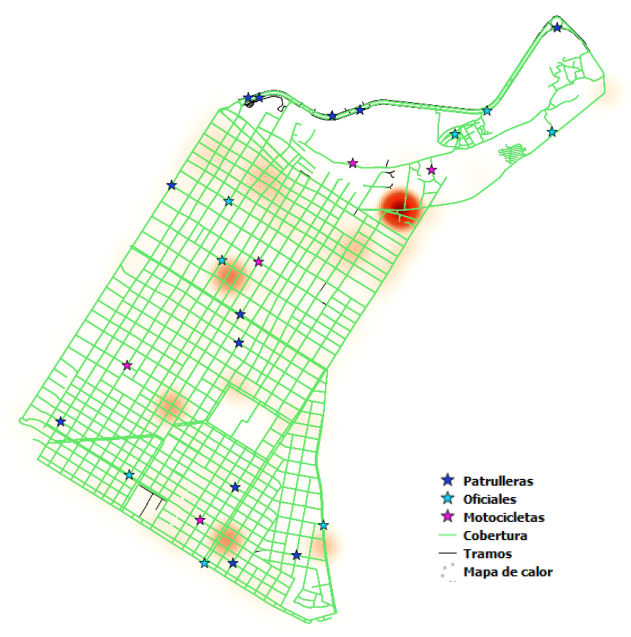
\includegraphics[width=90mm,scale=0.5]{images/estocastico_leyenda.png}}
        \subfigure[Búsqueda Tabú]{\label{fig:tabusearch}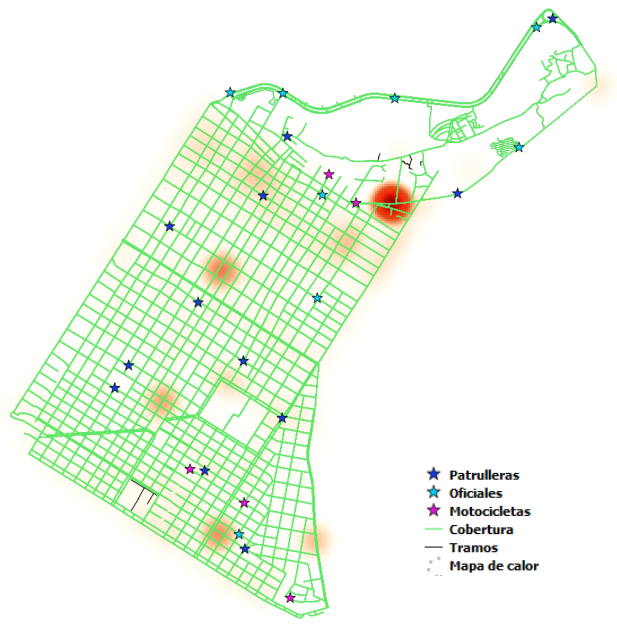
\includegraphics[width=90mm,scale=0.5]{images/tabusearch_leyenda.png}}
    \end{center}
    \caption{Mapas de cobertura por método}
    \label{fig:mapas-cobertura}
\end{figure}